\documentclass[12pt, a4paper]{article}

\usepackage[utf8]{inputenc}
\usepackage[T2A]{fontenc}
\usepackage[russian]{babel}
\usepackage[dvips]{graphicx}

\usepackage[oglav,spisok,boldsect,eqwhole,figwhole,hyperref,hyperprint,remarks,greekit]{./style/fn2kursstyle}
\graphicspath{{./style/}{./figures/}}
\usepackage{float}
\usepackage{multirow}
\usepackage{supertabular}
\usepackage{multicol}
\usepackage{hhline}
\usepackage{listings}
\usepackage{color}
\usepackage{adjustbox}
\usepackage{amsmath}
\usepackage{verbatim}

\definecolor{dkgreen}{rgb}{0,0.6,0}
\definecolor{gray}{rgb}{0.5,0.5,0.5}
\definecolor{mauve}{rgb}{0.58,0,0.82}

\lstset{frame=tb,
	language=C++,
	aboveskip=1mm,
	belowskip=1mm,
	showstringspaces=false,
	columns=flexible,
	basicstyle={\small},
	numbers=left,
	numberstyle=\tiny\color{gray},
	keywordstyle=\color{red},
	commentstyle=\color{dkgreen},
	stringstyle=\color{mauve},
	breaklines=true,
	breakatwhitespace=true,
	tabsize=2
}
\title{Численное решение краевых задач для одномерного уравнения теплопроводности \\ Варианты 5, 16}


%\authorfirst{О.\,Д.~Климов}
%\authorsecond{О.\,Д.~Климов} TODO: прописать команды в style.sty

\supervisor{С.\,А.~Конев}
\group{ФН2-61Б}
\date{2024}

%\renewcommand{\vec}[1]{\text{\mathversion{bold}${#1}$}}%{\bi{#1}}
\newcommand\thh[1]{\text{\mathversion{bold}${#1}$}}
\renewcommand{\labelenumi}{\theenumi)}
\renewcommand{\labelenumi}{\theenumi)}

\newcommand{\opr}{\textbf{\underline{{Опр.}}}\quad}
\newcommand{\theorem}{\textbf{\underline{{Теор.}}}\quad}
\renewcommand{\phi}{\varphi}
\renewcommand{\k}[1]{\textbf{\textit{#1}}}

\newcounter{mycounter}
\newcommand{\quastion}[1]{%
	\stepcounter{mycounter}%
	\textbf{\themycounter}.  %
	\textbf{\textit{#1}}
	
}

\newcommand{\rusg}{\text{Г}}

\begin{document}
	\maketitle
	\section{Ответы на контрольные вопросы}
	
	\quastion{Дайте определения терминам: корректно поставленная задача, понятие аппроксимации дифференциальной задачи разностной схемой, порядок аппроксимации, однородная схема, консервативная схема, монотонная схема, устойчивая разностная схема (условно/абсолютно), сходимость.}
	
	Пусть мы рассматриваем задачу о нахождении решения уравнения $Au = f$ в области $G$ с дополнительными условиями $Ru = \mu$ на границе $\rusg = \partial G$ области $G$:
	\begin{equation}
		Au = f   \text{ в } \, G, \quad Ru = \mu \text{ на } \rusg.
		\label{1}
	\end{equation}
	где $A$, $R$ --- заданные операторы, $f$,$\mu$ --- заданные функции.
	
	\opr \textbf{Задача} называется \textbf{корректно поставленной}, если ее решение существует, единственно и непрерывно зависит от входных данных. Если же не выполнено хотя бы одно из этих условий, то задача называется некорректно поставленной.
	
	\opr Функция, определённая только в узлах сетки, называется сеточной.
	
	\opr Построение разностной схемы --- это замена уравнений и дополнительных условий исходной задачи алгебраическими уравнениями для сеточных функций. Производные в исходных уравнениях заменяют конечными разностями, интегралы --- квадратурными формулами, прочие члены --- алгебраическими соотношениями.
	
	Пусть для точной задачи \eqref{1} используется разностная схема
	\begin{equation}
		A_h y = \phi   \text{ в } \, G_h, \quad R_h y = \nu \text{ на } \Gamma_h.
		\label{2}
	\end{equation}
	Сеточные функции $\psi_h = (\phi - f_h) + ((A v)_h - A_h v_h)$, \quad $\chi_h = (\nu - \mu_h) + ((R v)_h - R_h v_h)$ --- \textbf{погрешности аппроксимации разностной} задачи в~$G_h$ и~на~$\Gamma_h$ соответственно ($v$ есть произвольная функция из области определения оператора $A$).
	
	\opr Говорят, что \textbf{разностная схема аппроксимирует исходную задачу}, если $ ||\psi_h||_\psi \to 0$, $ ||\chi_h||_\chi \to 0$ при $h \to 0$. Аппроксимация имеет \textbf{\textit{p}-й порядок} ($p > 0$), если $ ||\psi_h||_\psi = O(h^p)$, $ ||\chi_h||_\chi = O(h^p)$  при $h \to 0$.
	
	\opr Разностные схемы называются \textbf{консервативными}, если их решение удовлетворяет дискретному аналогу закона сохранения (баланса), присущему данной задаче. В противном случае схему называют \textbf{неконсервативной}, или дисбалансной.
	
	\opr Разностные схемы, в которых расчет ведется по одним формулам и на одном шаблоне во всех узлах сетки без какого-то либо специального выделения имеющихся особенностей, называются \textbf{однородными}. 
	
	\opr Схемы, решение которых удовлетворяет принципу максимума или сохраняет пространственную монотонность(в одномерном случае) при условии, что соответствующие свойства справедливы для исходных задач, называются \textbf{монотонными}. 
	
	Пусть $y_1$, $y_2$ --- решения двух задач с одинаковым оператором, соответствующие правым частям $\phi_1$, $\phi_2$ и граничным условиям $\nu_1$, $\nu_2$.
	
	\opr Говорят, что \textbf{разностная схема устойчивая}, если решение уравнений схемы непрерывно зависит от входных данных и эта зависимость равномерна по $h$, т.е.
	\begin{equation*}
		\forall \varepsilon > 0 \phantom{x}\exists \delta(\varepsilon) > 0: \quad \parallel \phi_1 - \phi_2 \parallel_\phi < \delta,   \parallel \nu_1 - \nu_2 \parallel_\nu <  \delta \Rightarrow \parallel y_1 - y_2 \parallel_Y < \varepsilon
	\end{equation*}	
	
	\opr В случае нескольких независимых переменных \textbf{устойчивость} называют \textbf{безусловной}(или \textbf{абсолютной}), если устойчивость имеет место для любого соотношения шагов, и \textbf{условной} в противном случае.
	
	Будем различать следующие устойчивости. Устойчивость по правой части: непрерывная зависимость решения разностной задачи от $\phi$. Устойчивость по граничным условиям: непрерывная зависимость решения разностной задачи от $\nu$ на границе пространственной области. Устойчивость по начальным данным: непрерывная зависимость решения разностной задачи от $\nu$ на гиперплоскости $t=0$.
	
	\opr Разностное решение $y$ сходится к решению $u$ точной задачи, если \\
	\mbox{$\| y - p_h u \|_Y \to 0$} при $h \to 0$. Говорят, что имеет место \textbf{сходимость} с \textit{p}-м ($p > 0$) порядком, если $\| y - p_h u \|_Y = O(h^p)$ при $h \to 0$.
	
	\textsl{Замечание.} $f(x) = O(g(x)) \Leftrightarrow \forall x \in U(x): |f(x)| \le C|g(x)|$.
	
	
	\clearpage % для удобства редактирования <-> потом убрать
	\quastion{Какие из рассмотренных схем являются абсолютно устойчивыми? Какая из рассмотренных схем позволяет вести расчеты с более крупным шагом по времени?}
	
	Рассматриваем задачу с переменными коэффициентом температуропроводности $k=k(x,t)$:
	\[
	\begin{cases}
		u_t = (ku_x)_x, \phantom{xxx} 0<x<l, \phantom{xxx} 0<t<T; \\
		u(x,0) = u_0(x), \\
		u(0,t)=\mu_1(t), \phantom{xxx} u(l,t)=\mu_2(t).
	\end{cases}
	\]
	
	Для такой задачи в лабораторной работе рассматривается схема с весами вида:
	
	\begin{equation*}
		c \rho \frac{y^{j+1}_i - y^{j}_i}{\tau} = \frac{1}{h} (\sigma(a_{i+1} y^{j+1}_{x,i} - a_{i} y^{j+1}_{\bar{x},i}) + (1-\sigma)(a_{i+1} y^{j}_{x,i} - a_{i} y^{j}_{\bar{x},i}).
	\end{equation*}
	
	Запишем её в более компактном виде:
	\[
	y_t = (ay^{(\sigma)}_{\bar{x}}))_x,
	\]
	где $0<a_{min} \le a \le a_{max}$. 
	
	Вычисления проводим на равномерной сетке. Для анализа устойчивости воспользуемся методом энергетических неравенств. 
	
	Если операторы $A$ и $B$ не зависят от $t$, $A=A^*>0$ и $B=B^*>0$, то разностная схема $By_t+Ay=0$ устойчива по начальным данным в норме $\|\cdot\|_{A}=\{(A\cdot, \cdot)\}^{1/2}$, если $B\ge \frac{\tau}{2}A$.
	
	А метод энергетических неравенств основывается на приведённом выше утверждении и заключается в следующем.	
	Пусть $A=A^*>0$ и $B=B^*>0$ и $B\ge \frac{\tau}{2}A$. Тогда схема  $By_t+Ay=0$ устойчива по начальным данным.
	
	Заметим, что
	\[
	y^{(\sigma)} =(1-\sigma)y + \sigma \hat{y}= y + \sigma\tau \frac{\hat{y}-y}{\tau}= y+\tau \sigma y_t.
	\]
	
	Тогда схему с весами можно записать в виде:
	\[
	y_t = a y_{\bar{x}x}+\sigma\tau a y_{\bar{x}xt};
	\]
	\[
	(y-\sigma\tau a y_{\bar{x}x})_t = a y_{\bar{x}x}.
	\]
	
	Сравнивая схему со схемой $By_t+Ay=0$, получим, что в нашем случае:
	\[
	Ay = - y_{\bar{x},x}, \phantom{xxx} B = E+\tau\sigma A.
	\]
	Надо показать, что $E+\tau\sigma A \ge \frac\tau2 A$.
	
	Воспользуемся известной оценкой собственных значений задачи Штурма-Лиувилля в дискретном случае. То есть для задачи
	\[
	\begin{cases}
		-y_{\bar{x},x} = \lambda^2y,\\
		y_0 = 0, \phantom{xxx} y_n = 0
	\end{cases}
	\] 
	знаем, что $\dfrac{9}{l^2} \le \lambda^2_k \le \dfrac{4}{h^2}$.
	
	Отсюда можно сделать вывод, что для нашего случая
	\[
	\dfrac{9a_{min}}{l^2}\|y\|^2_2 \le (Ay,y) \le \dfrac{4a_{max}}{h^2}\|y\|^2_2.
	\]
	
	\[
	E \ge \tau(\frac{1}{2}-\sigma)A;
	\]
	A --- положительно определённый оператор, тогда
	\[
	1 \ge \tau \dfrac{4a_{max}}{h^2}(\frac12 - \sigma);
	\]
	\[
	\sigma \ge \dfrac12 - \dfrac{h^2}{4a_{max}\tau}.
	\]
	
	Из этой оценки получаем, что схема должна удовлетворять условию устойчивости для всего интервала изменения $a$, реализуемого в задаче. То есть на практике выбираем фиксированное значение $a$, исследуем схему на устойчивость при это значении параметра. После этого выбираем $\sigma$-вес, что удовлетворяет всему интервалу изменения $a$.
	
	Однако сделаем замечания. Данный приём называется ,,принцип замороженных коэффициентов''. Он, вообще говоря, является нестрогим, но часто даёт нужные результаты (не для всех схем). Так как $a(x,t)$ является непрерывной функцией, то её значения на достаточно большом разбиении отрезка в двух соседних пространственных узлах одного временного слоя мало различимы (нет разрыва), то можно считать в этой окрестности $a$ постоянным коэффициентом. И тогда можно провести исследование на $a_{max}$, выбрать устойчивую конфигурацию (выбрать нужные $\tau$, $h$,$\sigma$). Получим некую устойчивость ,,с запасом'' для случаев $a < a_{max}$.    
	
	
	\clearpage % для удобства редактирования <-> потом убрать
	\quastion{Будет ли смешанная схема иметь второй порядок аппроксимации при $a_i = \frac{2 K(x_i) K(x_{i-1})}{K(x_i) + K(x_{i-1})}$?}
	
	% ХЗ верно ли: Вариант исследования схемы, где мы приводим ее к формуле симпсона, но мне она кажется неверной из-за того, что подрузамеватся, что $h = x_i - x_{i+1}$, в то время как в методичке полагается $h = x_{i- 0.5} - x_{i+0.5} $
	\begin{comment}
		Имем однородную консервативную схему 
		\begin{equation*}
			c \rho \frac{y^{j+1}_i - y^{j}_i}{\tau} = \frac{1}{h} (\sigma(a_{i+1} y^{j+1}_{i+\frac{1}{2}} - a_{i} y^{j+1}_{i-\frac{1}{2}}) + (1-\sigma)(a_{i+1} y^{j}_{i+\frac{1}{2}} - a_{i} y^{j}_{i-\frac{1}{2}})),
		\end{equation*}
		где $a_i = \displaystyle{(\frac{1}{h}\int_{x_{i-1}}^{x_i} \frac{dx}{K(x)})^{-1}}$.
		
		%%% $ c \rho \frac{y^{j+1}_i - y^{j}_i}{\tau} = \frac{1}{h} (\sigma(\omega^{j+1}_{i+\frac{1}{2}} - \omega^{j+1}_{i-\frac{1}{2}}) + (1-\sigma)(\omega^{j}_{i+\frac{1}{2}} - \omega^{j}_{i-\frac{1}{2}}))$
		 
		Пусть $a_i = \frac{2 K(x_i) K(x_{i-1})}{K(x_i) + K(x_{i-1})}$. Тогда из равенства $\frac{2 K(x_i) K(x_{i-1})}{K(x_i) + K(x_{i-1})} = \displaystyle{(\frac{1}{h}\int_{x_{i-1}}^{x_i} \frac{dx}{K(x)})^{-1}}$ получим, что
		\begin{equation*}
			\int_{x_{i-1}}^{x_i} \frac{dx}{K(x)} = h \frac{2 K(x_i) K(x_{i-1})}{K(x_i) + K(x_{i-1})} = \frac{h}{2} (\frac{1}{K(x_{i-1})} + \frac{1}{K(x_{i})}).
		\end{equation*}
		Можно увидеть, что выражение является формулой трапеций, которая, как известно, имеет второй порядок точности. Следовательно рассмотренный случай также имеет 2 порядок.
	\end{comment}
	
	Имеем однородную консервативную схему 
	\begin{equation*}
		c \rho \frac{y^{j+1}_i - y^{j}_i}{\tau} = \frac{1}{h} (\sigma(a_{i+1} y^{j+1}_{x,i} - a_{i} y^{j+1}_{\bar{x},i}) + (1-\sigma)(a_{i+1} y^{j}_{x,i} - a_{i} y^{j}_{\bar{x},i}),
	\end{equation*}
	Преобразовав данное в вопросе выражение, имеем
	\begin{equation*}
		\frac{1}{a_i} = \frac{1}{2} \left( \frac{1}{K_i} + \frac{1}{K_{i-1}} \right)
	\end{equation*}
	
	
	Разложим в ряд Тейлора в окрестности точки $x_{i-\frac{1}{2}} = x_i - \frac{h}{2}$:
	\begin{equation*}
		\frac{1}{K_i} = \frac{1}{K_{i-\frac{1}{2}}} - \frac{2 K'_{i-\frac{1}{2}}}{(K_{i-\frac{1}{2}})^2} \frac{1}{2!} \frac{h}{2} + O(h^2), \quad
		\frac{1}{K_{i-\frac{1}{2}}} = \frac{1}{K_{i-\frac{1}{2}}} + \frac{2 K'_{i-\frac{1}{2}}}{(K_{i-\frac{1}{2}})^2} \frac{1}{2!} \frac{h}{2} + O(h^2)
	\end{equation*}
	Подставим и получим
	\begin{equation*}
	\frac{1}{a_i} = \frac{1}{2} \left( \frac{1}{K_i} + \frac{1}{K_{i-1} } + O(h^2)\right) = \frac{1}{K_{i-\frac{1}{2}}} + O(h^2)  \quad \Rightarrow \quad a_i = K_{i-\frac{1}{2}} + O(h^2)
	\end{equation*}
	Следовательно при $K_{i-\frac{1}{2}}$ получаем порядок аппроксимации $O(h^2)$.
	
	
	
	
	\clearpage % для удобства редактирования <-> потом убрать
	\quastion{Какие методы (способы) построения разностной аппроксимации граничных условий (2.5), (2.6) с порядком точности $O(\tau + h^2)$, $O(\tau^2 + h^2)$, $O(\tau + h)$ вы знаете?}
	
	Граничные условия (2.5), (2.6) являются граничными условиями 2-го рода. Погрешность аппроксимации граничных условий задаёт погрешность всего метода.
	
	Рассмотрим уравнение вида
	$
	u_t = (k u_x)_x
	$
с граничными условиями второго рода (например, слева):
\[
	-ku_x + \alpha u = p(t), \phantom{xxx} x = 0.
\]

Один из способов аппроксимации граничного условия --- непосредственно записать дифференциальные операторы через разностные соотношения:
\[
-k \dfrac{\hat{y}_1 - \hat{y}_0}{h} + \alpha \hat{y}_0 = \hat{p}.
\]

В таком случае
\[
\psi_h = \hat{p} - \alpha\hat{u}_0 + k\dfrac{\hat{u}_1-\hat{u}_0}{h} =  \hat{p} - \alpha\hat{u}_0 + \dfrac{k}{h} (\hat{u}_0 +h\hat{u}_{x,0}+\dfrac{h^2}{2}\hat{u}_{xx,0}-\hat{u}_0+O(h^3))=
\]
\[
= \hat{p} - \alpha\hat{u}_0 + k\hat{u}_{x,0} + O(h) = 0 + O(h).
\]

Однако, первый порядок по пространству нас может не устроить, если, например, мы применяем схему $y_t = k\hat{y}_{\bar{x},x}$ с порядком точности $O(\tau+h^2)$. Решим эту проблему, применив интегро-интерполяционный метод.
\[
\int_{t_j}^{t_{j+1}}\int_{x_0}^{x_{\frac12}} u_t dx dt =  \int_{t_j}^{t_{j+1}}\int_{x_0}^{x_{\frac12}} (ku_x)_x dx dt;
\]
\[
\int_{x_0}^{x_{\frac12}} (\hat{u}_0 - u_0) dx = \int_{t_j}^{t_{j+1}} ((ku_x)|_{x_{\frac12}}-(ku_x)|_{x_{0}})dt.
\]
Заменяем операторы разностными аналогами и учитываем граничные условия.
\[
\dfrac{\hat{y}_0-y_0}{\tau}\tau \dfrac{h}{2} = k\tau \dfrac{\hat{y}_1-\hat{y}_0}{h} + \tau \hat{p} - \tau \alpha \hat{y}_0;
\]
Домножаем обе части уравнения на $\dfrac h2$:
\[
y_{t,0} = \frac2h(k\hat{y}_{x,0} + \hat{p}-\alpha\hat{y}_0).
\]
В таком случае:
\[
\psi_h =-\frac h2 u_{t,0} + \hat{p} - \alpha \hat{u}_0 + k \dfrac{\hat{u}_1-\hat{u}_0}{h} = O(h^2).
\]
Причём, получили безусловную аппроксимацию. 

Помимо интегро-интерполяционного метода можно использовать и аппроксимацию ENO и WENO (взвешенные, существенно не осциллирующие схемы, в которых аппроксимация будет происходить с помощью кубического полинома).

%Пусть $f(u) = -ku_x$. Тогда уравнение теплопроводности можно записать в виде $u_t + F(u)_x=0$. 

	\clearpage % для удобства редактирования <-> потом убрать
	\quastion{При каких $h$, $\tau$ и $\sigma$ смешанная схема монотонна? Проиллюстрируйте результатами расчетов свойства монотонных и немонотонных разностных схем.}
		
	Рассматриваем схему с весами:
	\[
	c \rho \frac{y^{j+1}_i - y^{j}_i}{\tau} = \frac{1}{h} (\sigma(a_{i+1} y^{j+1}_{x,i} - a_{i} y^{j+1}_{\bar{x},i}) + (1-\sigma)(a_{i+1} y^{j}_{x,i} - a_{i} y^{j}_{\bar{x},i}).
	\]
	Для определения монотонности схемы будем проверять выполнение для неё условия положительности коэффициентов.
	
	\[
	c \rho \frac{y^{j+1}_i - y^{j}_i}{\tau} = \frac{1}{h^2} (\sigma(a_{i+1}(y^{j+1}_{i+1} -  y^{j+1}_{i}) - a_{i}(y^{j+1}_i - y_{i-1}^{j+1})) + (1-\sigma)(a_{i+1} (y^{j}_{i+1}-y^{j}_{i}) - a_{i} (y^{j}_i - y_{i-1}^{j}));
	\]
	
	\begin{multline*}
			(\dfrac{\sigma(a_{i+1}+a_i)}{h^2}+\frac{c \rho}{\tau})y_i^{j+1} = \dfrac{\sigma a_{i+1}}{h^2}y_{i+1}^{j+1} + \dfrac{\sigma a_{i}}{h^2}y_{i-1}^{j+1} + \frac{(1-\sigma)a_{i+1}}{h^2}y_{i+1}^j + \frac{(1-\sigma)a_{i}}{h^2}y_{i-1}^j +\\ 
			+(\frac{c \rho}{\tau} - \frac{(1-\sigma)(a_{i+1}+a_i)}{h^2})y_i^j.
	\end{multline*}
	
	Условие положительности коэффициентов можно записать в виде системы неравенств.
	\[
	\begin{cases}
			A = \dfrac{\sigma(a_{i+1}+a_i)}{h^2}+\dfrac{c \rho}{\tau} > 0,\\
			B_1 = \dfrac{\sigma a_{i+1}}{h^2} > 0,\\
			B_2 = \dfrac{\sigma a_{i}}{h^2} > 0,\\
			B_3 = \dfrac{(1-\sigma)a_{i+1}}{h^2} > 0,\\
			B_4 = \dfrac{(1-\sigma)a_{i}}{h^2} > 0,\\
			B_5 = \dfrac{c \rho}{\tau} - \dfrac{(1-\sigma)(a_{i+1}+a_i)}{h^2} > 0,\\
			D = A - \sum_{i=1}^{5}B_i \ge 0.
	\end{cases}
	\]

Известно, что $\sigma \in (0,1) \Rightarrow \sigma > 0$; $\rho > 0$; $c > 0$; $K(x) > 0 \Rightarrow a_i > 0$; $h>0$; $\tau>0$.
Из условия $B_5 > 0$ следует:
\[
\dfrac{c \rho}{\tau}  > \dfrac{(1-\sigma)(a_{i+1}+a_i)}{h^2};
\]
\begin{equation}
\label{ineq}
\dfrac{h^2}{\tau(1-\sigma)} > \dfrac{(a_{i+1}+a_i)}{c \rho};
\end{equation}

Соотношение $(a_{i+1}+a_i)$ определяется из способа вычисления $a_i$. Таким образом, схема, для которой неравенство \eqref{ineq} выполнено, является монотонной.

Приведём иллюстрации монотонного и немонотонного расчёта. Рассмотрим алюминиевый стержень длины 1 м. Согласно ГОСТ 22233-83 имеем следующие параметры: $\rho = 2600\frac{\text{кг}}{\text{м}^3}$, $c = 840 \frac{\text{Дж}}{\text{кг К}}$. Коэффициент $K = 221\frac{\text{Вт}}{\text{м К}}$ будем считать постоянным. Зададим начальное распределение температуры:
\[
u(x, 0) = u_0-500-x(L-x), \phantom{xxx} x\in(0, L),
\]
где $u_0=800$К. На концах стержня будем поддерживать постоянную температуру $u_0$. Расчёт будет вести до момента времени $T=100$с. 

Так как $K=const$, получаем $a_{i+1}+a_i = 221 + 221 = 442$.При выборе параметров схемы $h=0.05$, $\tau = 0.009$ и $\sigma = 0.5$:
\[
\dfrac{0.05^2}{0.009(1-0.5)} > \dfrac{442}{840\cdot 2600};
\]
\[
\dfrac59 > \frac{17}{84000} \Rightarrow \text{У.П.К. выполнено и схема монотонна}.
\]

 \begin{figure}[H]
	\centering
	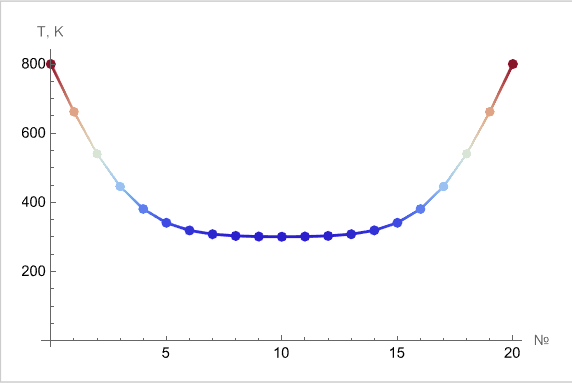
\includegraphics[width=1\textwidth]{monotExample}
	\caption{Распределение температуры в стержне при \mbox{$t=100$с} (монотонная схема)}
\end{figure}

\pagebreak

Нарушим монотонность схемы, выбрав значения $h=0.05$, $\tau = 14$, $\sigma = 0$.

 \begin{figure}[H]
	\centering	
	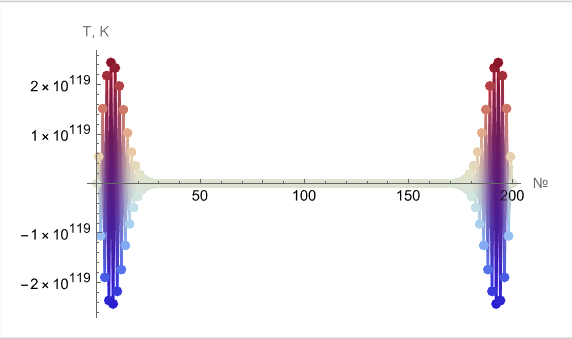
\includegraphics[width=1\textwidth]{nomonotExample}
	\caption{Распределение температуры в стержне при \mbox{$t=100$с} (немонотонная схема)}
\end{figure}

	\clearpage % для удобства редактирования <-> потом убрать
	\quastion{Какие ограничения на $h$, $\tau$ и $\sigma$ накладывают условия устойчивости прогонки?}
	
		Рассмотрим схему с весами:
	\[
	c \rho \frac{y^{j+1}_i - y^{j}_i}{\tau} = \frac{1}{h} (\sigma(a_{i+1} y^{j+1}_{x,i} - a_{i} y^{j+1}_{\bar{x},i}) + (1-\sigma)(a_{i+1} y^{j}_{x,i} - a_{i} y^{j}_{\bar{x},i}).
	\]
	
	Из полученного ранее:
	\begin{multline*}
		(\dfrac{\sigma(a_{i+1}+a_i)}{h^2}+\frac{c \rho}{\tau})y_i^{j+1} = \dfrac{\sigma a_{i+1}}{h^2}y_{i+1}^{j+1} + \dfrac{\sigma a_{i}}{h^2}y_{i-1}^{j+1} + \frac{(1-\sigma)a_{i+1}}{h^2}y_{i+1}^j + \frac{(1-\sigma)a_{i}}{h^2}y_{i-1}^j +\\ 
		+(\frac{c \rho}{\tau} - \frac{(1-\sigma)(a_{i+1}+a_i)}{h^2})y_i^j.
	\end{multline*}
	
	Домножим обе части равенства на $h^2$ и соберём неизвестные слагаемые слева.
	
	\begin{multline*}
	\dfrac{\sigma a_i}{h} y_{i-1}^{j+1} - (\dfrac{\sigma a_i}{h} + \dfrac{\sigma a_{i+1}}{h}+\dfrac{c \rho h}{\tau})y_i^{j+1} + \dfrac{\sigma a_{i+1}}{h} y_{i+1}^{j+1} = \\
	= - \frac{(1-\sigma)a_{i+1}}{h}y_{i+1}^j - \frac{(1-\sigma)a_{i}}{h}y_{i-1}^j -
	(\frac{c \rho h}{\tau} - \frac{(1-\sigma)(a_{i+1}+a_i)}{h})y_i^j.
\end{multline*}
	
	С помощью аппроксимации граничных условий получаем явное выражение для $y_0^{j+1}$ и $y_N^{j+1}$ (при условии $N$ шагов по пространству). Таким образом, перед нами --- система линейный алгебраических уравнений с трёхдиагональной матрицей.
	\[
	a_i  y_{i-1}^{j+1} - b_i y_i^{j+1} + c_i y_{i+1}^{j+1} = - d_i, \phantom{xxx} 0\le i\le N; \phantom{xxx} a_0=c_N = 0.
	\]
	 Хотелось бы применить для её разрешения метод прогонки, например, правой.
	
	\textbf{Теорема.} Если в трёхдиагональной матрице выполнено условие диагонального преобладания: $|b_i| \ge |a_i| + |c_i|$, где хотя бы для одного $i$ выполнено строгое неравенство, то исходная система уравнений имеет решение, которое может быть получено с помощью метода прогонки. Алгоритм прогонки в указанных условиях является корректным и устойчивым (все знаменатели прогоночных коэффициентов не обращаются в нуль, и все $|a_i| \le1$).
	
	В таком случае, для устойчивости прогонки необходимы следующие условия на параметры схемы.
	
	Для $i=1, \ldots, N-1$:
	\[
	|\dfrac{\sigma a_i}{h} + \dfrac{\sigma a_{i+1}}{h}+\dfrac{c \rho h}{\tau}| \ge |\dfrac{\sigma a_i}{h}| + |\dfrac{\sigma a_{i+1}}{h}|
	\]
	Из положительности коэффициентов $c$, $\rho$, $\tau$, $h$ и $\sigma$ следует, что условие диагонального преобладания выполнены, причём мы можем заявить о строгом неравенстве.
	
	Для $i=\alpha$, где $\alpha \in \{0, N\}$:
	\begin{enumerate}
		\item Случай граничного условия первого рода (постоянная температура на границе):
		\[
		y_\alpha^{j+1} = u_0 \Rightarrow 
		a_\alpha = 0, b_\alpha = 1, c_\alpha = 0, d_\alpha = u_0 \Rightarrow \text{У.Д.П. выполнено.}
		\]
		
		\item Случай граничного условия второго рода (заданный поток на границе):
		\[
		y_\alpha^{j+1} = \varkappa^{(\alpha)} y_{\alpha - \text{sign}(\alpha-1)}^{j+1} + \mu^{(\alpha)} ,
		\]
		где $\varkappa^{(\alpha)} = 
		\begin{cases}
			 \frac{\sigma a_1 /h}{c\rho h/(2\tau) + \sigma a_1/h}, \phantom{xxx} \alpha = 0\\
			 \frac{\sigma a_N /h}{c\rho h/(2\tau) + \sigma a_N/h}, \phantom{xxx} \alpha = N
		\end{cases}$;
	
	\[
	\mu^{(\alpha)} = \begin{cases}
		\dfrac{\sigma P(t_{j+1})+(1-\sigma)(w_{\frac12}^j + P(t_j)) + \frac{c \rho h}{2\tau}y_0^j}{c\rho h / (2\tau) + \sigma a_1/h}, \phantom{xxx} \alpha = 0\\
		\dfrac{\sigma P(t_{j+1})+(1-\sigma)(P(t_j)-w_{N-\frac12}^j) + \frac{c \rho h}{2\tau}y_N^j}{c\rho h / (2\tau) + \sigma a_N/h}, \phantom{xxx} \alpha = N
	\end{cases}.
	\]
	
	Тогда $a_{\alpha}= \begin{cases}
		0,& \phantom{xx} \alpha = 0,\\
		\varkappa^{(N)},& \phantom{xx} \alpha = N
	\end{cases}$;
	$b_{\alpha}= 1$; 
	$c_{\alpha}= \begin{cases}
		\varkappa^{(0)},& \phantom{xx} \alpha = 0,\\
		 0,& \phantom{xx} \alpha = N
	\end{cases}$; 
	$d_{\alpha}= \mu^{(\alpha)}$. 
	
	Для выполнения У.Д.П. необходимо:
	\[
	1 \ge |a_{\alpha} + c_{\alpha}|; 
	\]
	\[
	\begin{cases}
		1 \ge \left|\varkappa^{(0)}\right|,& \phantom{xx} \alpha = 0,\\
		1 \ge \left|\varkappa^{(N)}\right|,& \phantom{xx} \alpha = N.\\
	\end{cases};
	\]
	\[
	\begin{cases}
		1 \ge \left| \frac{\sigma a_1 /h}{c\rho h/(2\tau) + \sigma a_1/h}\right|,& \phantom{xx} \alpha = 0,\\
		1 \ge \left| \frac{\sigma a_N /h}{c\rho h/(2\tau) + \sigma a_N/h}\right|,& \phantom{xx} \alpha = N.\\
	\end{cases};
	\]
	
	Таким образом, получили необходимые соотношения.
	\end{enumerate}
	
	
	\clearpage % для удобства редактирования <-> потом убрать
	\quastion{В случае $K = K(u)$ чему равно количество внутренних итераций, если итерационный процесс вести до сходимости, а не обрывать после нескольких первых итераций?}
	
	\textbf{Тест 1}. Поставим задачу квазилинейного уравнения теплопроводности:
	\[
	\begin{cases}
		c \rho \dfrac{\partial u}{\partial t} = \dfrac{\partial}{\partial x}\left(K(u)\dfrac{\partial u}{\partial x} \right), \phantom{xxx} 0<x<L, \phantom{xxx} 0<t\le T, \\
		u(x,0) = \text{initState}(x), \phantom{xxx} 0<x<L,\\
		u(0,t) = u_0, \phantom{xxx} 0 \le t \le T,\\
		u(L, t) = u_0, \phantom{xxx} 0 \le t \le T,
	\end{cases}
	\]
	где $\rho = 2600\frac{\text{кг}}{\text{м}^3}$, $c = 840 \frac{\text{Дж}}{\text{кг К}}$, $u_0 = 800$К, $\text{initState}(x)=u0-500 - x(L-x)$, $L=1$м, $T=100$с, $K(u)=13.7+0.0017u+0.000003u^2$.
	
	Будем оценивать количество внутренних итераций эмпирически. Критерий сходимости $\|y^{s+1}-y^{s}\| < \varepsilon_i$, где $\varepsilon_i \in \{10^{-4},10^{-7},10^{-10}\}$. Число итераций на каждом временном слое для различных $\varepsilon_i$ представлены на рисунках ниже.
	
	 \begin{figure}[H]
		\centering
		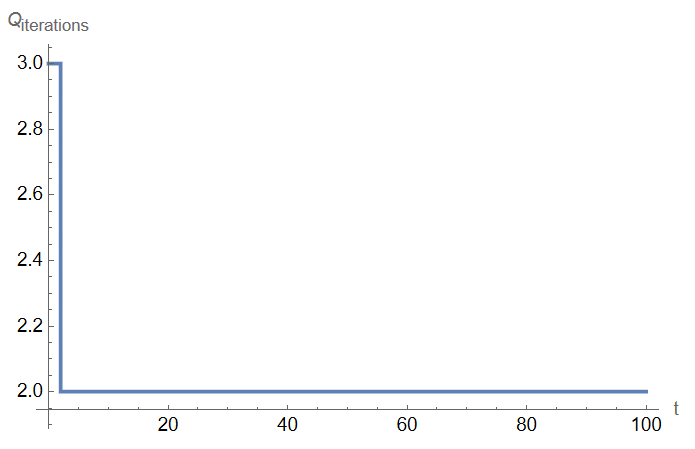
\includegraphics[width=1\textwidth]{test1-1e-4}
		\caption{Тест 1, $\varepsilon_i=10^{-4}$}
	\end{figure}

 \begin{figure}[H]
	\centering
	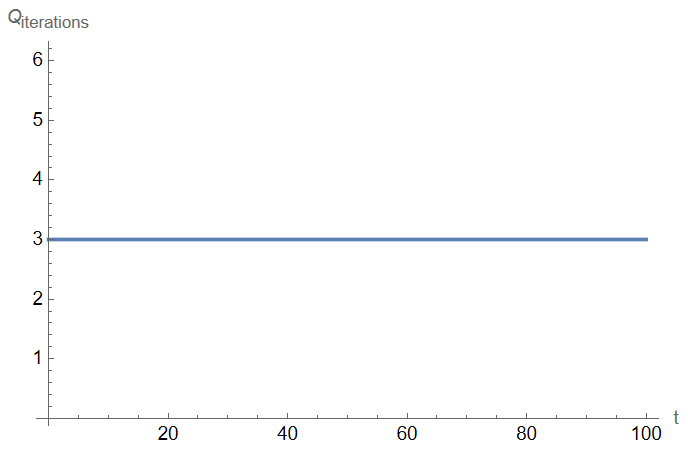
\includegraphics[width=1\textwidth]{test1-1e-7}
	\caption{Тест 1, $\varepsilon_i=10^{-7}$}
\end{figure}
	
	 \begin{figure}[H]
		\centering
		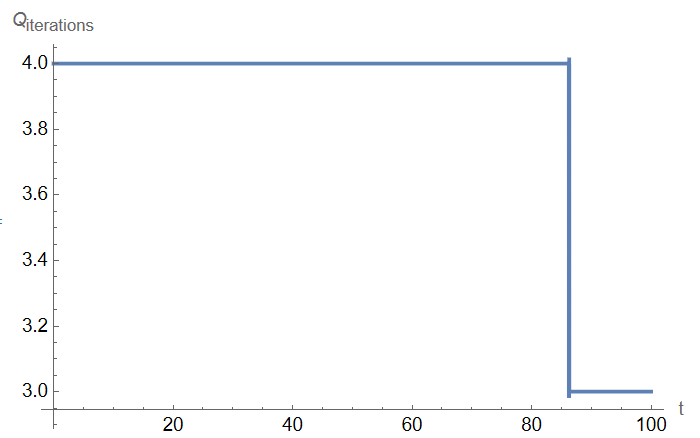
\includegraphics[width=1\textwidth]{test1-1e-10}
		\caption{Тест 1, $\varepsilon_i=10^{-10}$}
	\end{figure}
	
	

	\textbf{Тест 2}. Рассмотрим также задачу следующего вида:
		\[
	\begin{cases}
		\dfrac{\partial u}{\partial t} = \dfrac{\partial}{\partial x}\left(0.5\cdot u^2\dfrac{\partial u}{\partial x} \right), \phantom{xxx} 0<x<L, \phantom{xxx} 0<t\le T, \\
		u(x,0) = 0, \phantom{xxx} 0<x<L,\\
		u(0,t) = \sqrt{\dfrac{2\cdot5^2}{0.5}}t^{\frac12}, \phantom{xxx} 0 \le t \le T,\\
		K(u)\dfrac{\partial u}{\partial x}|_{(L,t)}=0, \phantom{xxx} 0 \le t \le T,
	\end{cases}
	\]
	
	Расчёты будем проводить с шагами $h=0.2$, $\tau=2\cdot 10^{-4}$. Выберем $L=10$, $T=1$.  Критерий сходимости $\|y^{s+1}-y^{s}\| < \varepsilon_i$, где $\varepsilon_i \in \{10^{-4},10^{-7},10^{-10}\}$. Число итераций на каждом временном слое для различных $\varepsilon_i$ представлены на рисунках ниже.
	
	 \begin{figure}[H]
		\centering
		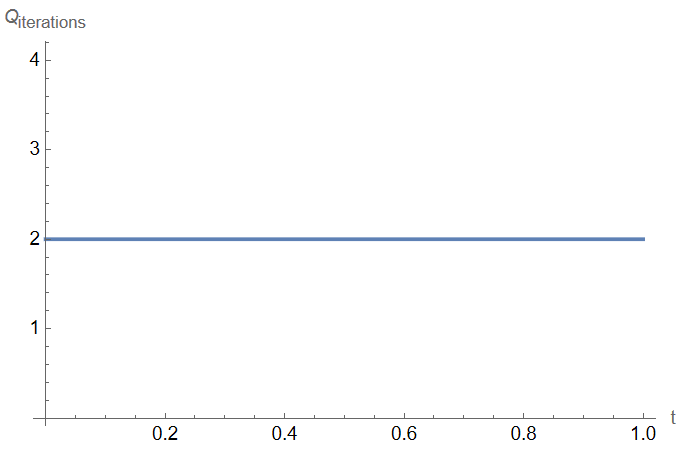
\includegraphics[width=1\textwidth]{test3-1e-4}
		\caption{Тест 2, $\varepsilon_i=10^{-4}$}
	\end{figure}
	
	\begin{figure}[H]
		\centering
		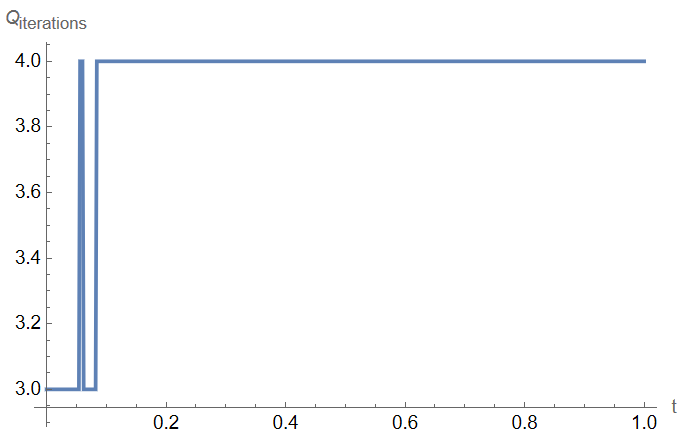
\includegraphics[width=1\textwidth]{test3-1e-7}
		\caption{Тест 2, $\varepsilon_i=10^{-7}$}
	\end{figure}
	
	\begin{figure}[H]
		\centering
		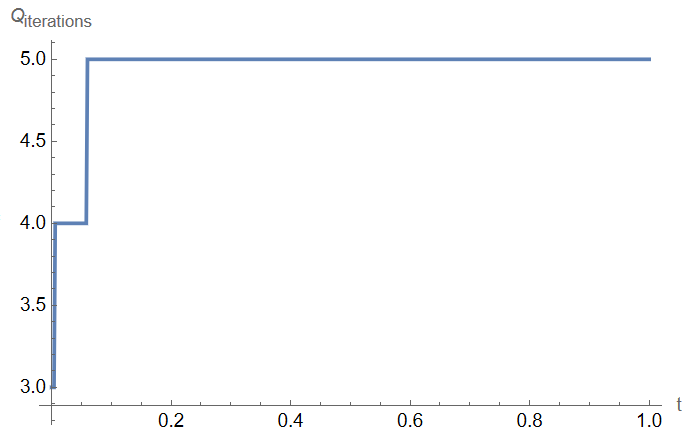
\includegraphics[width=1\textwidth]{test3-1-e-10}
		\caption{Тест 2, $\varepsilon_i=10^{-10}$}
	\end{figure}
	
	
	\clearpage % для удобства редактирования <-> потом убрать
	\quastion{Для случая K = K(u) предложите способы организации внутреннего итерационного процесса или алгоритмы, заменяющие его.}
	
	В статье \cite{5} предлагается алгоритм решения квазилинейного уравнения теплопроводности, основанный на использовании явной разностной схемы. Зависимость коэффициентов уравнения от температуры преодолевается введение новой искомой функции --- первообразной теплопроводности.
	
	Авторы предлагают уравнение
	\[
		с \rho\dfrac{\partial u}{\partial t} = \dfrac{\partial}{\partial x}\left(K(u)\dfrac{\partial u}{\partial x} \right)
	\]
	заменой 
	\[
	G(u) = \int_{0}^{u} K(\xi)d\xi
	\]
	получить уравнение
	\[
	\dfrac{\partial G}{\partial t} = a^2(u)\dfrac{\partial^2G}{\partial x^2},
	\]
	где $a(u) = \sqrt{K(u)/(c\rho)}$ --- коэффициент температуропроводности. Функция $G(u)$ является строго монотонной функцией температуры.
	
	Шаблон разностной схемы предлагается выбрать следующим:
	\[
	\dfrac{dG_i(t)}{dt} = a^2(u_i) \dfrac{G_{i-1}(t)-2G_i(t)+G_{i+1}(t)}{h^2}, \phantom{xxx} t\in[0, \tau], \phantom{x} i=2,\ldots,N-1.
	\]
	
	Аппроксимация значений $G_{i-1}(t)$ и $G_{i+1}(t)$ с точностью до членов первого порядка малости даёт следующую схему
	\[
	\dfrac{dG_i(t)}{dt} + \dfrac{2a^2(u_i)}{h^2}G_i(t) = \dfrac{a^2(u_i)}{h^2}\left( G_{i-1}(0) + G_{i+1}(0) + \big(\dfrac{dG_{i-1}(t)}{dt}(0)+\dfrac{dG_{i+1}(t)}{dt}(0)\big)t\right).
	\]
	
	Решением полученного уравнения является функция
	\[
		G_i(t) = (G_i(0)-B) \exp\{-\frac{2a^2(u_i)}{h^2}t\} + At + B, \phantom{xxx} t\in [0, \tau],
	\]
	где $A=\frac12 \big(\dfrac{dG_{i-1}(t)}{dt}(0)+\dfrac{dG_{i+1}(t)}{dt}(0)\big)$,
	\mbox{$B = \dfrac{G_{i-1}(0)+G_{i+1}(0)}{2}-A\cdot \dfrac{h^2}{2a^2(u_i)}$}.
	
	Записав разностные аппроксимации для производных по времени, 
	\[
	\dfrac{G_{i-1}}{dt}(0) = \frac{G_{i-1}^{(+\frac{1}{2})}-G_{i-1}^{(-\frac{1}{2})}}{\tau},
	\]
	\[
	\dfrac{G_{i+1}}{dt}(0) = \frac{G_{i+1}^{(+\frac{1}{2})}-G_{i+1}^{(-\frac{1}{2})}}{\tau},
	\]
	получим:
	\[
	G_i^{(+1)} = (G_i - B)\exp\{-\frac{2a^2(u_i)}{h^2}t\} + A\tau +B,
	\]
	где $A = \frac{1}{2\tau}(G_{i-1}^{(+\frac12)}  - G_{i-1}^{(-\frac12)} + G_{i+1}^{(+\frac12)} - G_{i+1}^{(-\frac12)})$, 
	\mbox{$B=\frac{G_{i-1}+G_{i+1}}{2} - A\cdot \frac{h^2}{2a^2(u_i)}$}.
	
	Для применения схемы необходимо по заданному значению $G_i$ найти температуру $u_i$ такую, что $G_i = \int_{0}^{u_i}q(\xi)d\xi$. В силу монотонности функции $G(u)$ эту задачу можно решить, например, методом дихотомии (деления отрезка пополам) или методом Ньютона.
	\clearpage
	\begin{thebibliography}{9}
		\bibitem{1} Галанин М.\,П., Савенков Е.\,Б. Методы численного анализа математических моделей. М.: Изд-во МГТУ им. Н.\,Э. Баумана, 2018. 592 с.
		\bibitem{2} Марчевский И.\,К., Щерица О.\,В. Численные методы решения задач математической физики: методические указания к выполнению лабораторных работ по курсу <<Методы вычислений>>. М.: Изд-во МГТУ им. Н.\,Э. Баумана, 2016. 63 с.
		\bibitem{3} Калиткин Н.\,Н.
		Численные методы: учеб. пособие. —
		2-е изд., исправленное. СПб.: БХВ-Петербург, 2011. 
		592 с. 
		\bibitem{4}  Y.-T. Zhang, C.-W. Shu ENO and WENO schemes, Handbook of Numerical Analysis, Volume 17, Handbook of Numerical Methods for Hyperbolic Problems: Basic and Fundamental Issues. North-Holland, Elsevier, Amsterdam, 2016.
		\bibitem{5} А.\,В. Геренштейн, М.\,З. Хайрисламов Явная разностная схема решения одномерного квазилинейного уравнения теплопроводности. Вестник ЮУрГУ. Серия: Математика. Механика. Физика. 2013. №1.
	\end{thebibliography}
	
\end{document}